%
% vektorprodukt.tex
%
% (c) 2018 Prof Dr Andreas Müller, Hochschule Rapperswil
%
\documentclass[tikz,12pt]{standalone}
\usepackage{times}
\usepackage{amsmath}
\usepackage{txfonts}
\usepackage[utf8]{inputenc}
\usepackage{graphics}
\usetikzlibrary{arrows,intersections,math}
\usepackage{ifthen}
\begin{document}

\newboolean{showgrid}
\setboolean{showgrid}{false}

\begin{tikzpicture}[>=latex,thick]

% Povray Bild
\node at (0,0) {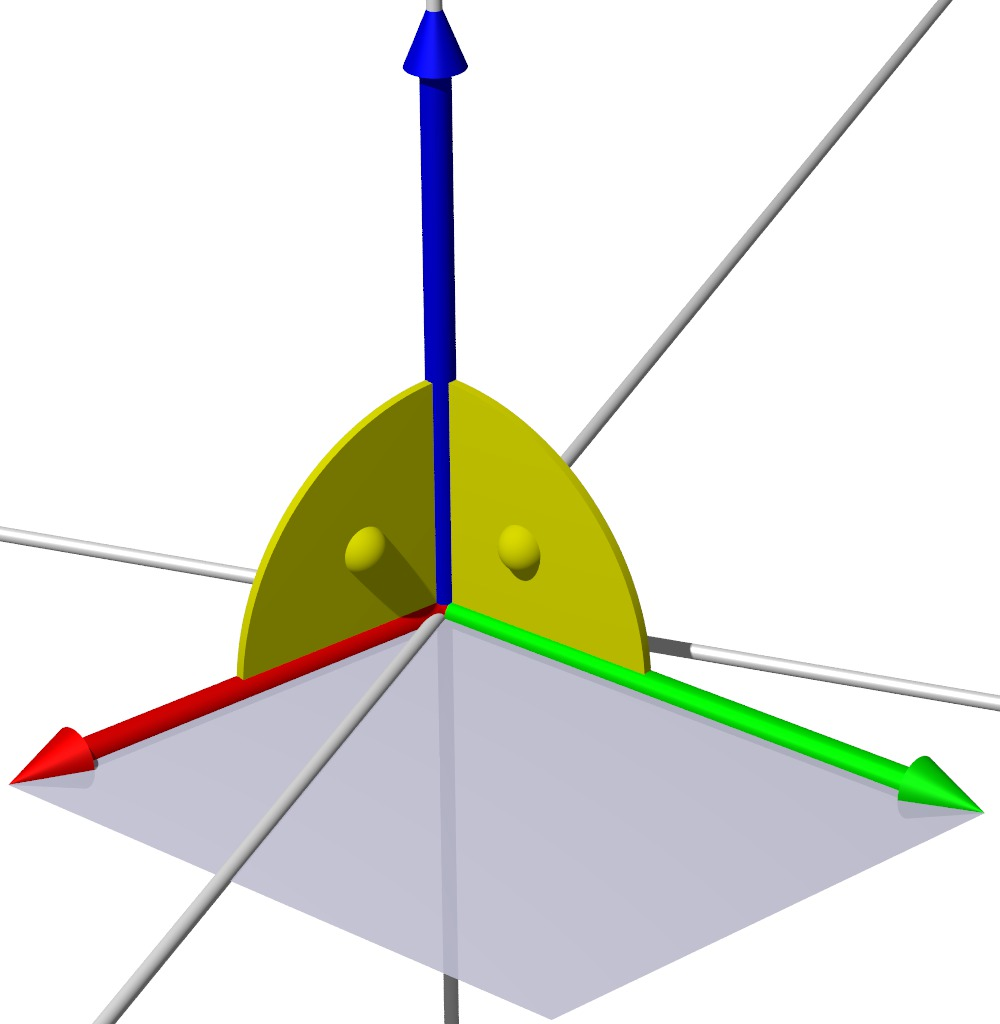
\includegraphics[width=8cm]{vektorprodukt.jpg}};

% Gitter
\ifthenelse{\boolean{showgrid}}{
\draw[step=0.1,line width=0.1pt] (-4,-4) grid (4, 4);
\draw[step=0.5,line width=0.4pt] (-4,-4) grid (4, 4);
\draw (-4,-4) grid (4, 4);
\fill (0,0) circle[radius=0.05];
}{}

% Vektoren
\node at (3.9,-2) {$\vec{b}$};
\node at (-3.8,-1.6) {$\vec{a}$};
\node at (0.1,4) {$\vec{a}\times\vec{b}$};

% Flaecheninhalt
\node at (0.3,-2.5) {$|\vec{a}\times\vec{b}|$};

% Nullpunkt
\node at (-0.2,-0.55) {$O$};

\end{tikzpicture}

\end{document}

